\documentclass{standalone} 
\PassOptionsToPackage{usenames,dvipsnames,svgnames}{xcolor}  
\usepackage{tikz}
\usetikzlibrary{arrows,positioning,automata}

\begin{document}
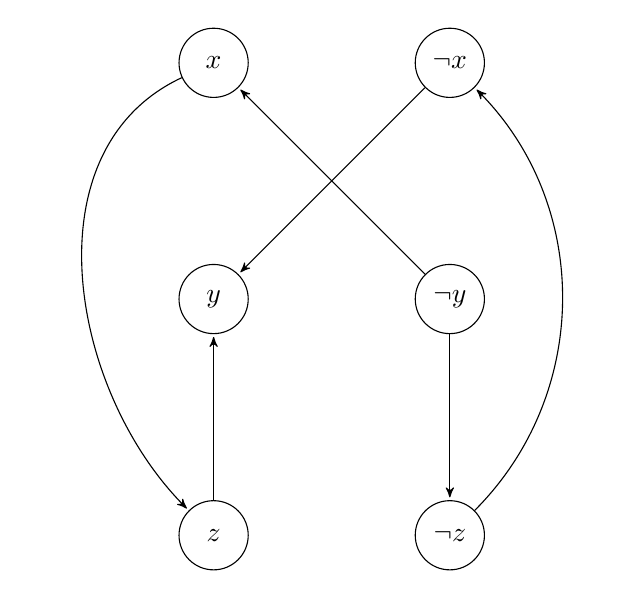
\begin{tikzpicture}[>=stealth',shorten >=1pt,node distance=3cm,on grid,initial/.style    ={}]
  \node[state]          (x)                         {$x$};
  \node[state]          (nx) [right = of x]    {$\neg x$};
  \node[state]          (y)  [below = of x]    {$y$};
  \node[state]          (ny) [right = of y]    {$\neg y$};
  \node[state]          (z)  [below = of y]    {$z$};
  \node[state]          (nz) [right = of z]    {$\neg z$};

  \path (ny)     edge [->]                    node   {} (x);
  \path (x)      edge [->, in=135, out=205]   node   {} (z);
  \path (z)      edge [->]                    node   {} (y);
  \path (nx)     edge [->]                    node   {} (y);
  \path (ny)     edge [->]                    node   {} (nz);
  \path (nz)     edge [->, in=-45, out=45]   node   {} (nx);
\end{tikzpicture}
\end{document}